\section{Basics}

This section describes the necessary basics for the hardware used in this project, as well as the operating system and the architecture behind the object detection.

\subsection{Robot Operating System (ROS)}
The Robot Operating System (ROS) is an open-source robotics meta-operating system for robots and as such provides hardware abstraction, low-level device control, message-passing between processes, and package management as well as tools and libraries for writing and running code across several computers \autocite{ros-intro}.

ROS consists of three concept levels, the file system level, the computation graph level, and the community level. The file system level covers things such as packages and the community level connects community members through different distributions and repositories. At the center is the computational graph, which is the peer-to-peer network for ROS processes consisting of nodes, master, parameter server, messages, services, topics, and bags. Nodes are processes that perform the computation, they communicate with each other by sending messages. Messages are subscribed to and published by topics. At the center the master takes care of registration and lookup, so nodes can find each other and exchange information --- as the below image shows \autocite{ros-concepts}.

\begin{figure}[!ht]
\centering
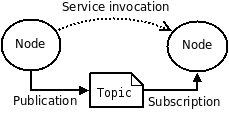
\includegraphics[width=4.5cm]{images/basics/ROS_basic_concepts.png}
\caption{ROS Basic Concepts \autocite{ros-concepts}}
\label{fig:ros-basic-concepts}
\end{figure}
% Source: http://ros.org/images/wiki/ROS_basic_concepts.png

\subsection{The TurtleBot3 Burger}
The TurtleBot3 Burger is part of the TurtleBot family of robots. It is a small, affordable, programmable, ROS-based mobile robot and can be used for research and prototyping \autocite{emanual-turtlebot3-ov}. The below pictures show the dimensions and components of the robot, as it is delivered by default.

\begin{figure}[!ht]
\centering
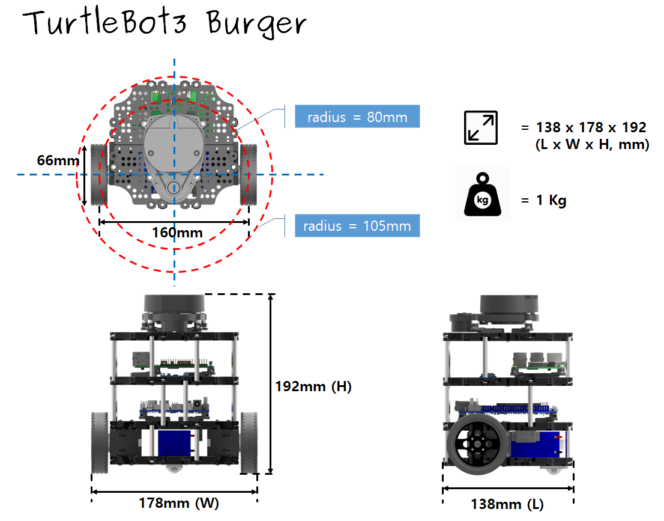
\includegraphics[width=\linewidth]{images/basics/turtlebot3_dimension1.png}
\caption{Turtlebot3 Burger Dimensions \autocite{emanual-turtlebot3-comp}}
\label{fig:turtlebot-dimensions}
\end{figure}
%Source: https://emanual.robotis.com/assets/images/platform/turtlebot3/hardware_setup/turtlebot3_dimension1.png

\begin{figure}[!ht]
\centering
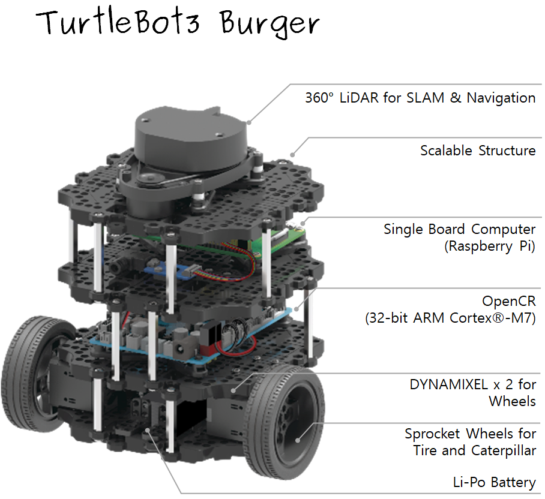
\includegraphics[width=\linewidth]{images/basics/turtlebot3_burger_components.png}
\caption{Turtlebot3 Burger Components \autocite{emanual-turtlebot3-comp}}
\label{fig:turtlebot-components}
\end{figure}
%Source: https://emanual.robotis.com/assets/images/platform/turtlebot3/hardware_setup/turtlebot3_burger_components.png

The complete specifications can be found in the official documentation. The LiDAR sensor is not used for this project.

\subsection{Object Detection}

The following subsections explain the basics of object detection, more specifically the \ac{YOLO} approach.

\subsubsection{YOLO}

While there are many approaches to object detection, the \ac{YOLO} approach stands out. When its paper was released back in 2015 it outperformed many of the existing detectors of that time. The full version is able to detect 45 frames per second and the fast version is detecting 155 frames per second with a Titan X graphics card on the PASCAL VOC dataset while still having more than double the \ac{mAP} than other real-time detectors in that comparison. Compared to its competitors it makes more localisation errors but has less false positives \autocite{yolo}.

\ac{YOLO} only looks once over an image. It consists of one single convolutional neural network that predicts bounding boxes and probabilities. This means that it treats object detection as a regression problem and predicts objects in one single go through in contrast to other detectors which mostly use pipelines with multiple stages \autocite{yolo}.
Unlike many other detectors, \ac{YOLO} does not use a sliding window approach or region proposal-based techniques but sees the complete image. This enables it to make use of contextual information about objects and to not see parts of the image isolated. Therefore it detects less false positives when mistaking background patches for objects. It learns a more generalized representation of objects and can more easily be applied to new domains than other detectors. The downside of this is that it is less accurate on small objects compared to other state-of-the-art systems.

\begin{figure}[!ht]
\centering
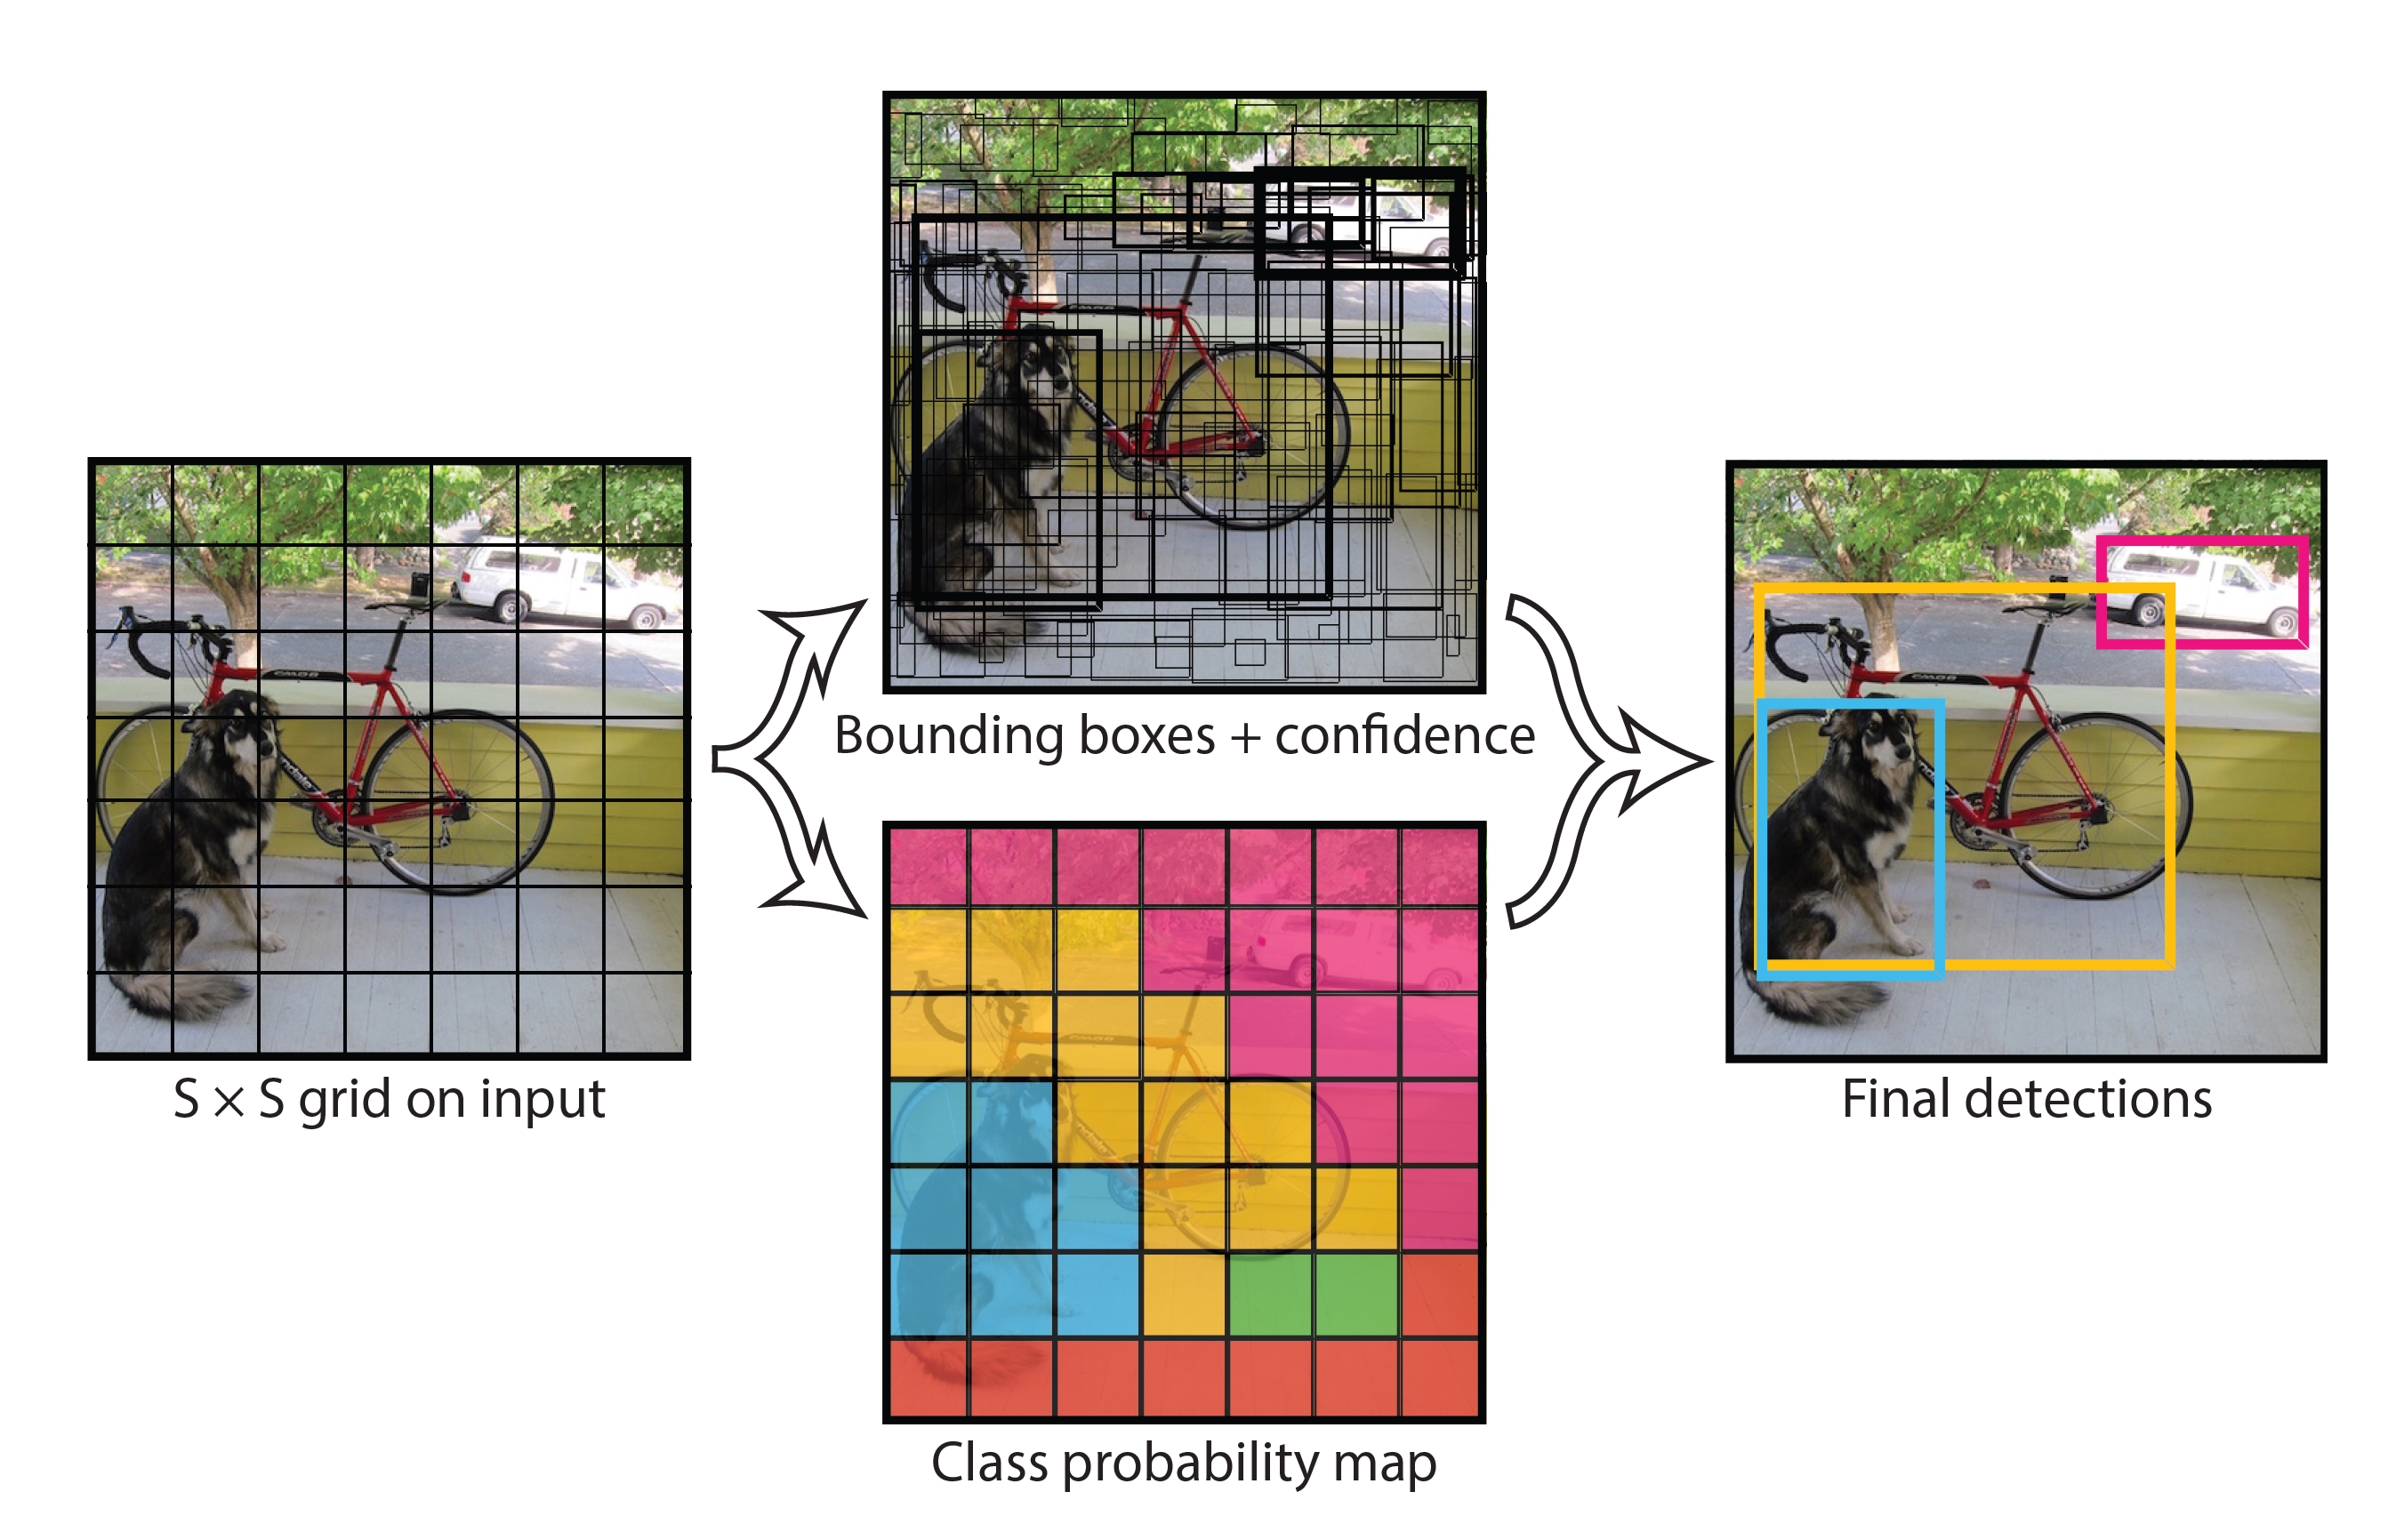
\includegraphics[width=\linewidth]{images/basics/yolo_detection_grid}
\caption{The image is divided into a grid for detecting features. \autocite{yolo}}
\label{fig:yolo_detection_grid}
\end{figure}

In \ac{YOLO} normally separated components for detecting objects are merged into one single neural network. The input image is divided into a \textit{S} x \textit{S} sized grid, where \textit{S} is the size of the grid (\autoref{fig:yolo_detection_grid}) \autocite{yolo}.

Each cell is responsible for detecting the object whose center is located in the corresponding cell. Every cell predicts \textit{B} bounding boxes and their confidence score. These predictions consist of \textit{x}- and \textit{y}-coordinates of the center, width, height and confidence of the bounding box. The confidence represents how confident the system is that the predicted bounding box matches the real object's bounds. Combined with conditional class probabilities a class specific confidence for each bounding box is calculated. These scores represent how likely the class matches the object and how likely the bounds match the bounds of the object (\autoref{fig:yolo_detection_grid}) \autocite{yolo}.

The neural network consists of 26 layers, 24 convolutional layers and two fully connected layers. The initial convolutional layers extract features from the image. To reduce the feature space alternating 1x1 layers are used with 3x3 layers (\autoref{fig:yolo_layers}) \autocite{yolo}.

\begin{figure}[!ht]
\centering
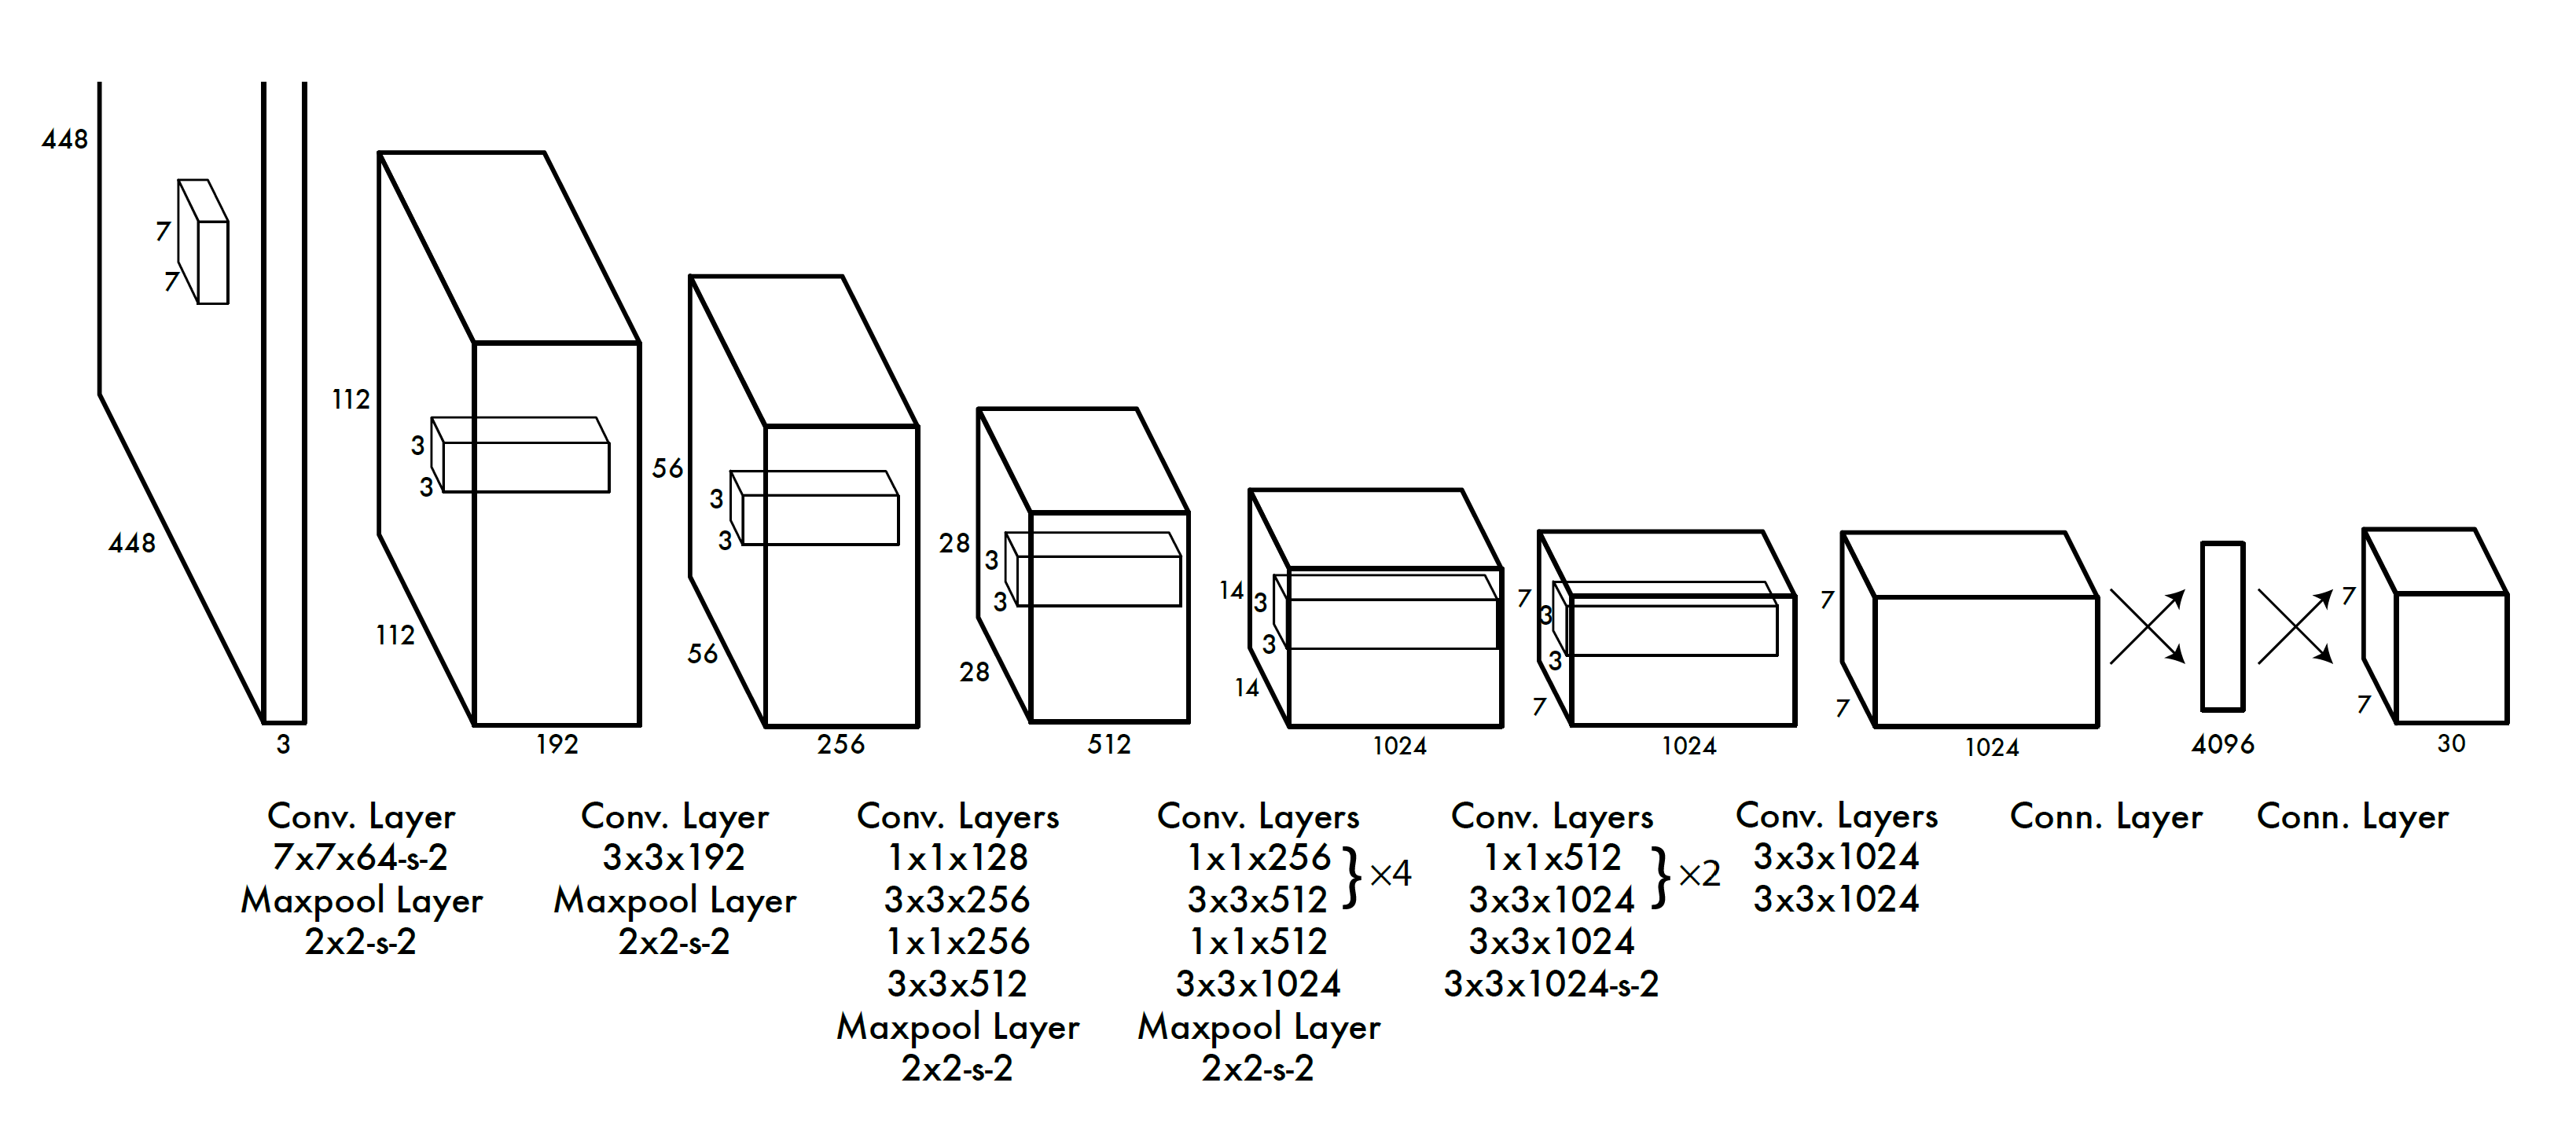
\includegraphics[width=\linewidth]{images/basics/yolo_layers}
\caption{Architecture of the network. \autocite{yolo}}
\label{fig:yolo_layers}
\end{figure}

The fully connected layers predict probabilities and coordinates of the bounding boxes. For the fast version only 9 convolutional layers are used. It is much faster than the full version but also less accurate \autocite{yolo}.

As the training of the network is not of importance in this project it will not be covered in this paper.

The \ac{YOLO} approach also has some limitations. As each cell only predicts two boxes it has problems with multiple objects close to each other, especially when they are small, a flock of birds for example. Objects with unusual aspect ratios are problematic too. Another problem is that the loss function during training treats errors in small and large boxes the same, but a small error in a small box has a much larger impact than a small error in a large box. This leads to incorrect localisations of objects \autocite{yolo}.

\subsubsection{YOLOv4}

As there currently is no paper on the newest version YOLOv5 the rough structure of YOLOv4 will be explained here.

\begin{figure*}[!ht]
\centering
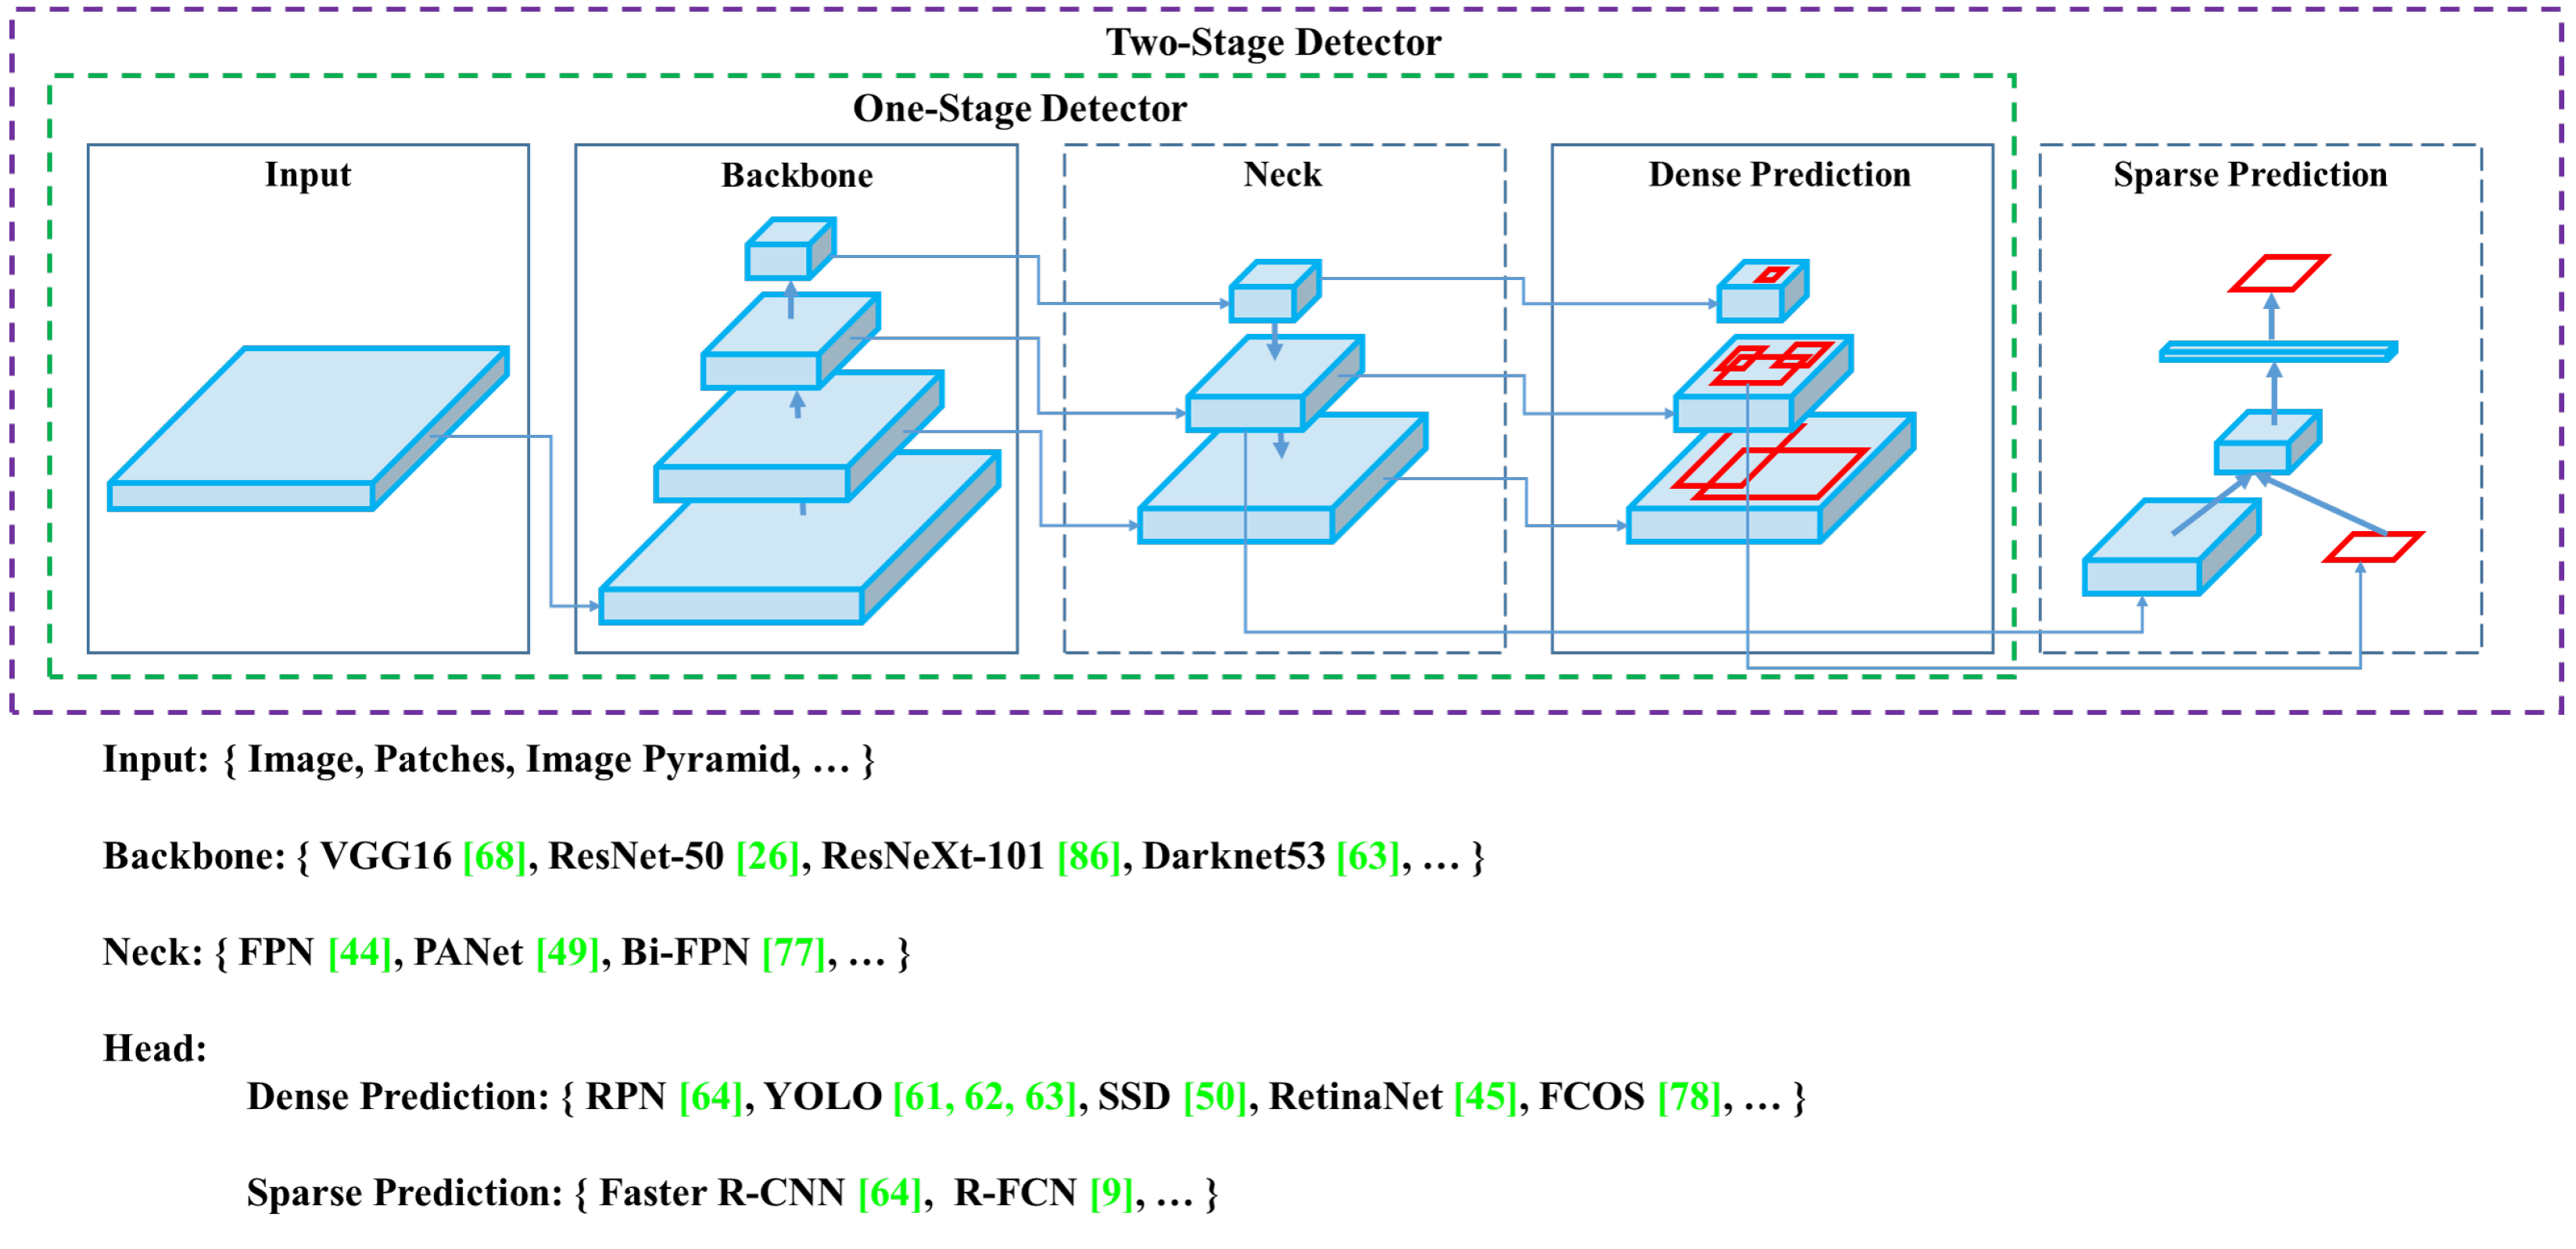
\includegraphics[width=\textwidth]{images/basics/yolov4_architecture}
\caption{Architecture of one- and two-stage object detectors. In the case of YOLOv4 we look at a one-stage detector. The sparse prediction part
therefore is irrelevant in this context. \autocite{yolov4}}
\label{fig:yolov4_architecture}
\end{figure*}

YOLOv4 consists of an input layer, a backbone, a neck and a head (\autoref{fig:yolov4_architecture}). The input layer is a standard input layer. The backbone consists of multiple convolutional layers that are responsible for extracting important features from the input image. The researchers chose the CSPDarknet53 neural network for this task. Following the backbone the neck generates feature pyramids from the extracted features. These pyramids generalize the object scaling. For this stage \ac{SPP} and \ac{PANet} were selected. \ac{SPP} increases the receptive field which describes the area that is looked at at once. A larger receptive field means that not only the object is evaluated but the area around it, therefore a larger context is included. \ac{SPP} separates out the most significant context features. The \ac{PANet} is used for parameter aggregation. Finally the head is used to predict classes and bounding boxes. In YOLOv4 the \ac{YOLO} approach is selected for this task, more precisely YOLOv3 \autocite{yolov4}.

\begin{figure}[!ht]
\centering
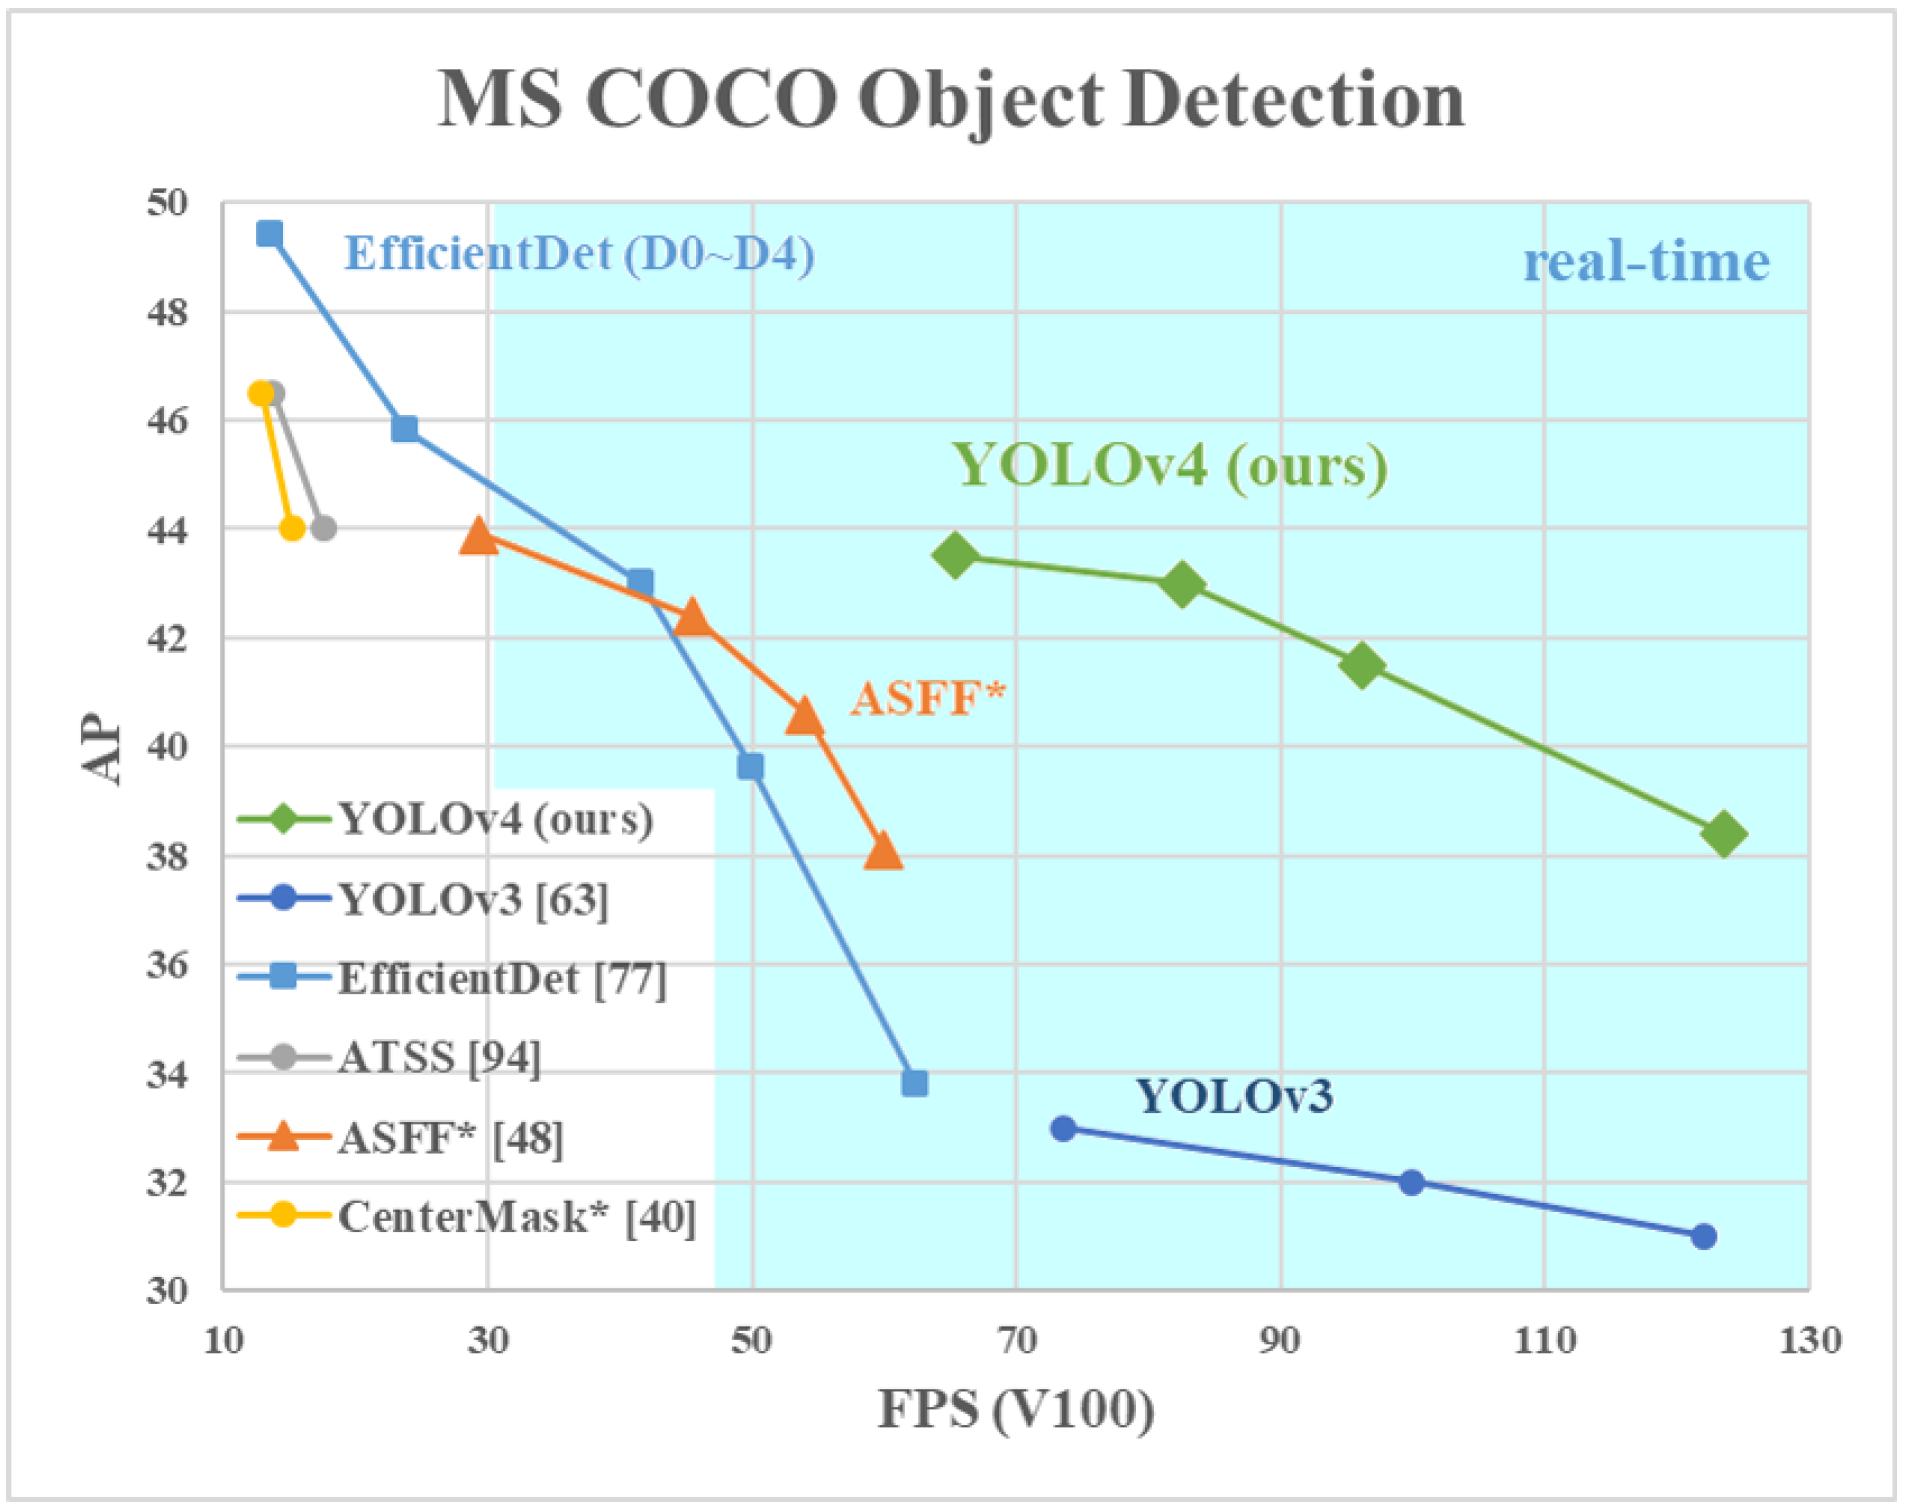
\includegraphics[width=\linewidth]{images/basics/yolo_v4_performance}
\caption{Performance comparison between YOLOv4, the predecessor YOLOv3 and other state-of-the-art detectors on the MS COCO dataset. \autocite{yolov4}}
\label{fig:yolo_v4_performance}
\end{figure}

As seen in \autoref{fig:yolo_v4_performance} YOLOv4 outperforms all other state-of-the-art detectors. Although EfficientDet, CenterMask and ATSS are able to perform better regarding the average precision they lack the speed of YOLOv4. YOLOv3 offers a comparable speed but at a much lower average precision. A more detailed comparison can be found at the researchers GitHub repository (https://github.com/AlexeyAB/darknet) \autocite{yolov4}.

\subsubsection{YOLOv5}

Although there currently is no paper on YOLOv5 the editorial team of TOWARDS AI published an article about its architecture.

YOLOv5 is a single-stage object detector too, so the rough overview of \autoref{fig:yolov4_architecture} can be applied. 
It consists of a backbone for feature extraction, a neck for feature pyramids that help with object scaling and unseen data and a head for predicting bounding boxes, classes and confidence. For the backbone the \ac{CSPNet} was selected, for the neck \ac{PANet} and for the head YOLOv3 again. In the hidden layers the Leaky ReLU function was selected as activation function, in the final detection layer a sigmoid function is used \autocite{towards_ai}.

\begin{figure}[!ht]
\centering
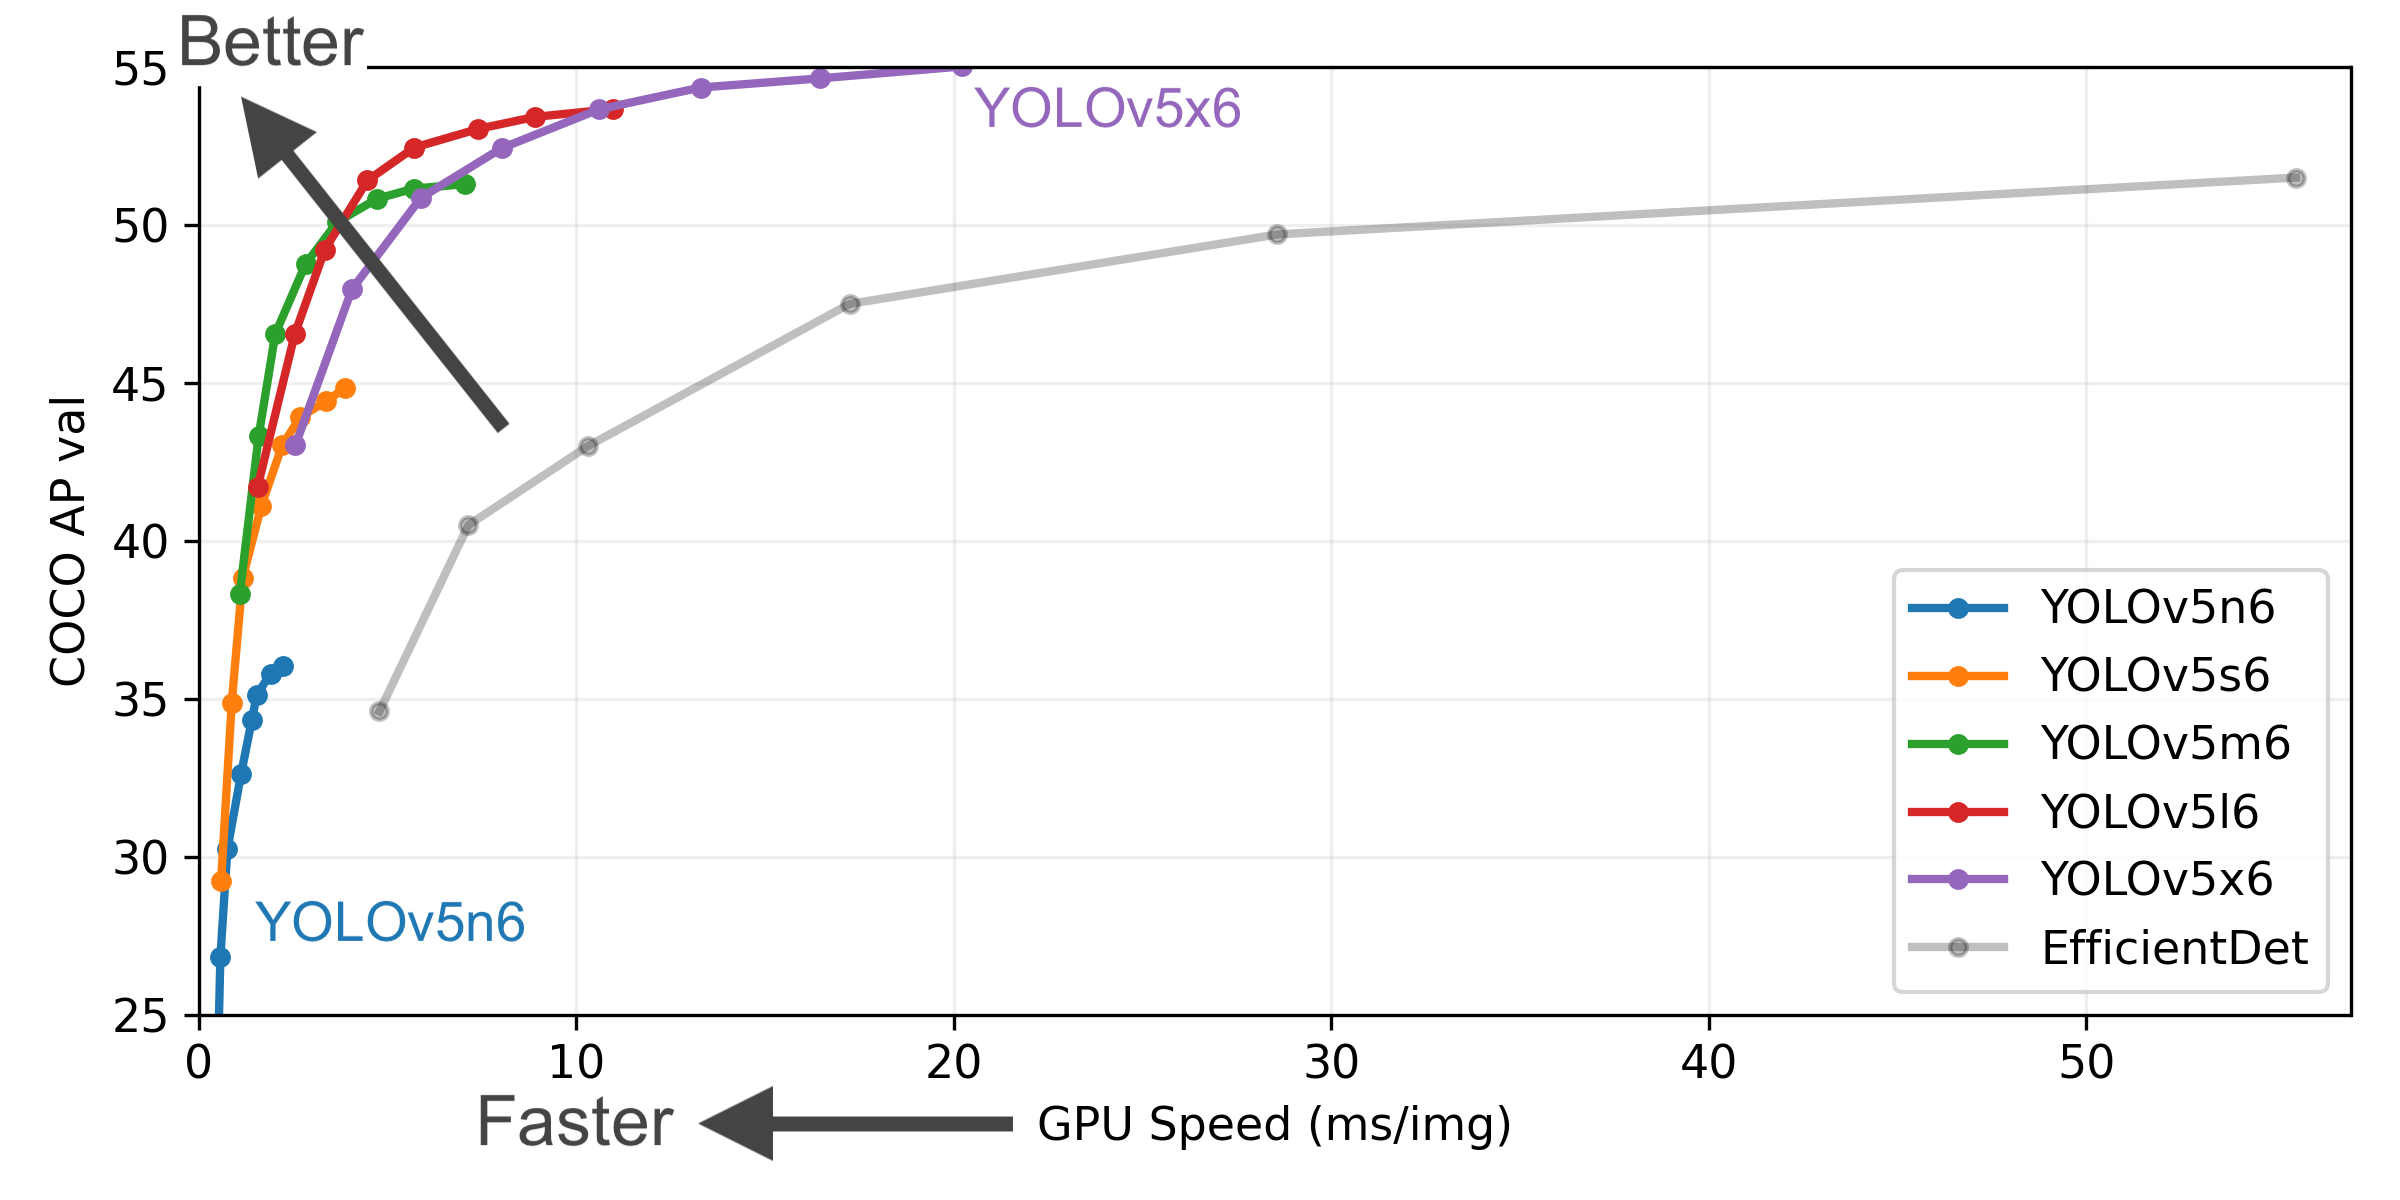
\includegraphics[width=\linewidth]{images/basics/yolov5_comparison}
\caption{Comparison between different YOLOv5 models and EfficientDet. It is important to notice that the x-axis is measured in milliseconds per image, not images per second as in \autoref{fig:yolo_v4_performance}. \autocite{ultralytics}}
\label{fig:yolov5_comparison}
\end{figure}

There are multiple pretrained models of YOLOv5 (YOLOv5n6, YOLOv5s6, YOLOv5m6, YOLOv5l6 and YOLOv5x6). The researchers of YOLOv5 show a performance comparison between the different YOLOv5 models and EfficientDet \autoref{fig:yolov5_comparison}). All YOLOv5 models perform faster than EfficientDet with some also having a better average precision \autocite{ultralytics}.

